\documentclass[12pt,oneside,a4paper]{report}

% --- Paquetes Básicos para Formato Profesional ---
\usepackage[utf8]{inputenc}
\usepackage[spanish,es-tabla]{babel}
\usepackage{geometry}
\geometry{top=3cm, bottom=3cm, left=3.5cm, right=2.5cm}
\usepackage{graphicx}
\usepackage{setspace}
\onehalfspacing
\usepackage{booktabs}
\usepackage{hyperref}
\renewcommand{\_}{\textunderscore\allowbreak}
\usepackage{listings}
\usepackage{xcolor}
\usepackage{tikz}
\usetikzlibrary{shapes.geometric, arrows.meta, positioning, fit, backgrounds}
\usepackage{amsmath}
\raggedbottom

% --- Configuración de listings para código Python ---
\lstdefinestyle{pystyle}{
    language=Python,
    basicstyle=\ttfamily\footnotesize,
    keywordstyle=\color{blue}\bfseries,
    stringstyle=\color{orange!80!black},
    commentstyle=\color{gray}\itshape,
    numberstyle=\tiny\color{gray},
    numbers=left,
    numbersep=8pt,
    breaklines=true,
    frame=single,
    rulecolor=\color{gray!40},
    backgroundcolor=\color{gray!5},
    captionpos=b,
    showstringspaces=false,
    tabsize=4,
}

\begin{document}

% ==========================================================
%                      PORTADA
% ==========================================================
\begin{titlepage}
    \centering
    {\scshape\Large Máster en Big Data y Análisis de Datos \par}
    \vspace{1cm}
    {\scshape\large Trabajo de Fin de Máster \par}
    \vspace{2.5cm}
    {\huge\bfseries Arquitectura de Datos en Tiempo Real y Modelado Predictivo de Retrasos Aeroportuarios mediante Redes Neuronales de Grafos \par}
    \vspace{0.5cm}
    {\large\itshape Integración en entornos híbridos y despliegue sobre Microsoft Fabric \par}
    \vspace{3.5cm}
    \begin{minipage}[t]{0.45\textwidth}
        \begin{flushleft} \large
            \emph{Autores:}\\
            Juan José Cecilla Morales\\
            Gonzalo López Crespo\\
            Alan Kroh
        \end{flushleft}
    \end{minipage}
    \hfill
    \begin{minipage}[t]{0.45\textwidth}
        \begin{flushright} \large
            \emph{Tutor:} \\
            José Ignacio Merino Martín\\
        \end{flushright}
    \end{minipage}
    \vfill
    \vspace{2cm}
    {\large Málaga, \today \par}
\end{titlepage}

% ==========================================================
%               DECLARACIÓN DE ORIGINALIDAD
% ==========================================================
\newpage
\thispagestyle{empty}
\chapter*{Declaración de Originalidad}
\vspace{1cm}

Nosotros, los abajo firmantes, declaramos que el presente Trabajo Fin de Máster, titulado \textit{`Arquitectura de Datos en Tiempo Real y Modelado Predictivo de Retrasos Aeroportuarios mediante Redes Neuronales de Grafos'}, es original y ha sido realizado por los miembros del equipo de manera íntegra.

Afirmamos que todas las fuentes consultadas, herramientas de computación y repositorios de datos utilizados se citan adecuadamente en el texto y en la sección bibliográfica, cumpliendo estrictamente con las normativas de integridad académica y propiedad intelectual del programa de postgrado.

\vspace{2.5cm}

\begin{center}
    \begin{tabular}{ccc}
        \underline{\hspace{5cm}} & \hspace{1cm} & \underline{\hspace{5cm}} \\
        Juan José Cecilla Morales & & Gonzalo López Crespo \\
        Socio del Proyecto & & Socio del Proyecto \\
        \vspace{1.5cm} \\
        & \underline{\hspace{5cm}} & \\
        & Alan Kroh & \\
        & Socio del Proyecto &
    \end{tabular}
\end{center}

% ==========================================================
%                        RESUMEN
% ==========================================================
\newpage
\thispagestyle{plain}
\begin{center}
    {\Large\bfseries Resumen \par}
\end{center}
\vspace{0.5cm}

La congestión y el retraso en las operaciones aéreas representan uno de los mayores desafíos económicos y logísticos para el sector de la aviación comercial a nivel global. Los enfoques predictivos tradicionales a menudo omiten la naturaleza relacional del tráfico aéreo, el cual se comporta intrínsecamente como una red interconectada de aeropuertos y rutas. Este Trabajo de Fin de Máster presenta el diseño e implementación de una solución integral de Big Data y analítica predictiva para la estimación de retrasos en tiempo real, combinando infraestructuras de computación distribuida con técnicas de aprendizaje profundo geométrico.

En primer lugar, se desarrolla una arquitectura de datos moderna estructurada en áreas funcionales optimizadas sobre el entorno de \textbf{Microsoft Fabric}, utilizando clústeres de \textbf{Apache Spark} para el procesamiento masivo de datos históricos de vuelo. El ciclo de ingesta en tiempo real se materializa mediante una \textbf{Azure Function} serverless (\texttt{GetFlightData}) que actúa como punto de entrada horario, remapeando datos históricos de 2022 a la hora corriente y escribiendo en tres zonas diferenciadas del Lakehouse. Para simular un entorno de producción continuo y solventar las restricciones críticas de memoria comunes en arquitecturas \textit{serverless}, se ha diseñado un pipeline de ingesta basado en una \textbf{ventana deslizante dinámica de 13 horas} ($T-5$ horas de contexto real a $T+8$ horas de horizonte predictivo). El núcleo predictivo está constituido por una \textbf{Red Neuronal de Grafos Secuencia a Secuencia (Seq2SeqGNN)} programada en PyTorch, la cual modela los aeropuertos como nodos y las rutas como aristas, capturando eficazmente la propagación espacio-temporal del retraso a lo largo de la red.

Los datos procesados y las inferencias generadas por el modelo de inteligencia artificial se consolidan en tablas de almacenamiento \textbf{Delta Lake}, permitiendo una explotación analítica optimizada en \textbf{Power BI} mediante el protocolo \textit{Direct Lake}. El cuadro de mandos interactivo final actúa como un centro de control operativo, ofreciendo segmentación por aeropuerto origen y un sistema de alertas tempranas tipo semáforo basado en umbrales de riesgo de negocio. Los resultados demuestran la viabilidad técnica de integrar GNNs en una arquitectura de datos distribuida de extremo a extremo: el modelo predice el retraso medio de llegada con un error absoluto medio (MAE) en torno a 10 minutos --- desde 9,1 minutos a una hora vista hasta 11,1 minutos a ocho horas vista ---, proporcionando una herramienta viable y escalable para la mitigación proactiva de contingencias en la gestión del tráfico aéreo.

\vspace{0.8cm}

% ==========================================================
%            SECCIÓN DE ÍNDICES
% ==========================================================
\pagenumbering{roman}
\setcounter{page}{3}

\pdfbookmark{\contentsname}{toc}
\tableofcontents
\newpage

\cleardoublepage
\listoffigures
\newpage

\cleardoublepage
\listoftables
\newpage

% ==========================================================
%       REINICIO DE NUMERACIÓN PARA EL CUERPO
% ==========================================================
\cleardoublepage
\pagenumbering{arabic}
\setcounter{page}{1}

% ==========================================================
%         CAPÍTULO 1: INTRODUCCIÓN Y OBJETIVOS
% ==========================================================
\chapter{Introducción y Objetivos}
\label{cap:introduccion}

\section{Motivación y Planteamiento del Problema}
\label{sec:motivacion}

La optimización de las cadenas de suministro y la gestión logística global dependen intrínsecamente de la puntualidad y la eficiencia de los sistemas de transporte. Dentro de las diferentes modalidades, el transporte aéreo comercial desempeña un papel crítico debido a su velocidad y capacidad para conectar nodos económicos distantes. Sin embargo, este sistema está expuesto a una variabilidad constante, donde los retrasos en los vuelos se erigen como uno de los problemas operativos más costosos y complejos de mitigar.

Desde la perspectiva de la gestión de operaciones, un retraso aéreo no constituye un evento aislado, sino que desencadena un efecto dominó a lo largo de toda la cadena de valor. Para las empresas dependientes de la logística ``justo a tiempo'' (\textit{Just-in-Time}), las desviaciones temporales en las horas programadas de llegada provocan consecuencias económicas severas, tales como la falta de abastecimiento de componentes críticos o la rotura de stock de inventarios estratégicos. Esta falta de predictibilidad impide a las organizaciones anticipar las contingencias, forzándolas a adoptar una postura reactiva que eleva los costes de almacenamiento de seguridad y merma la satisfacción del cliente final.

Para dar respuesta a esta problemática, surge la necesidad de diseñar e implementar herramientas tecnológicas avanzadas capaces de prever con precisión los retrasos aeroportuarios antes de que se consoliden en la red. No obstante, los enfoques predictivos tradicionales basados en series temporales estándar o modelos de regresión lineal y machine learning clásico (como Random Forest o Gradient Boosting generalistas) presentan severas limitaciones teóricas. Dichos modelos suelen tratar cada vuelo o cada aeropuerto como unidades de observación independientes, omitiendo la estructura subyacente y las interdependencias del sistema.

La realidad operativa demuestra que el tráfico aéreo funciona como un sistema dinámico fuertemente interconectado. Un retraso en un aeropuerto principal (\textit{hub}) como Chicago O'Hare (ORD) o John F. Kennedy (JFK) propaga inestabilidad de manera inmediata a los aeropuertos de destino a través de las aeronaves y tripulaciones compartidas.

Por ello, la tesis fundamental de este trabajo radica en que el espacio aéreo de los Estados Unidos puede ser modelado matemáticamente de manera exacta como un grafo topológico de gran escala, donde los aeropuertos representan los vértices o nodos, y las rutas comerciales constituyen las aristas o conexiones orientadas en el tiempo. Bajo este paradigma relacional, el uso de Redes Neuronales de Grafos (\textit{Graph Neural Networks}, GNN) se presenta como la metodología idónea. Las GNN permiten explotar el aprendizaje profundo geométrico para capturar simultáneamente los atributos locales de los vuelos (vientos, horarios, aerolíneas) y la estructura topológica global de la red, transformando la gestión reactiva tradicional en una estrategia de prevención logística proactiva y guiada por los datos.

\section{Objetivos del Proyecto}
\label{sec:objetivos}

\subsection{Objetivo General}
\label{sub:obj_general}

El objetivo general de este Trabajo de Fin de Máster es diseñar, desarrollar e implementar una arquitectura integral de Big Data y analítica predictiva en un entorno empresarial dinámico, capaz de modelar el tráfico aéreo de los Estados Unidos como una estructura de grafo e inferir con precisión los retrasos futuros de los vuelos mediante Redes Neuronales de Grafos (GNN), consolidando los resultados en un cuadro de mandos interactivo en tiempo real que optimice la toma de decisiones logísticas y prevenga la rotura de stock.

\subsection{Objetivos Específicos}
\label{sub:obj_especificos}

Para la consecución del objetivo general, se establecen los siguientes objetivos específicos divididos por áreas operativas:

\begin{itemize}
    \item \textbf{Ingeniería e Infraestructura de Datos:}
    \begin{itemize}
        \item Desplegar una infraestructura de almacenamiento y computación eficiente en el entorno cloud de \textbf{Microsoft Fabric}.
        \item Implementar una \textbf{Azure Function} serverless como mecanismo de ingesta horaria que actúe como puerta de entrada al Lakehouse, simulando un feed de datos en tiempo real a partir de registros históricos de 2022.
        \item Optimizar la ingesta de grandes volúmenes de datos históricos mediante el uso de conexiones desacopladas (\textit{Shortcuts}) a repositorios masivos en la nube.
        \item Desarrollar e implementar algoritmos optimizados en \textbf{Apache Spark} (PySpark) para estructurar y gestionar una \textbf{ventana deslizante dinámica de 13 horas}, simulando de manera controlada un entorno de producción en tiempo real.
    \end{itemize}

    \item \textbf{Ciencia de Datos y Modelado Predictivo:}
    \begin{itemize}
        \item Transformar el dataset estructurado de aviación en una representación matemática de grafo espacio-temporal, parametrizando los aeropuertos como nodos interconectados y las rutas comerciales como aristas dinámicas.
        \item Diseñar y entrenar una arquitectura avanzada de \textbf{Red Neuronal de Grafos Secuencia a Secuencia (Seq2SeqGNN)} capaz de capturar el ``efecto dominó'' y la propagación de los retrasos a lo largo de la red de transporte.
        \item Realizar un tratamiento estadístico de sesgos en la capa de datos corporativa, controlando anomalías operativas mediante el ajuste de minutos de retraso negativos a valores de negocio representativos.
    \end{itemize}

    \item \textbf{Inteligencia de Negocio y Visualización:}
    \begin{itemize}
        \item Construir un cuadro de mandos interactivo e integrado en \textbf{Power BI} utilizando la modalidad de conexión analítica \textit{Direct Lake} para asegurar consultas de alto rendimiento sin replicación de datos.
        \item Diseñar interfaces operativas que incluyan segmentación dinámica por aeropuerto de origen y monitorización continua del comportamiento temporalizado de los vuelos (Pasado vs. Futuro).
        \item Implementar un sistema predictivo visual de alertas tempranas mediante formatos condicionales automatizados (KPIs tipo semáforo), adaptados a las reglas de riesgo de la gestión de operaciones aeroportuarias.
    \end{itemize}
\end{itemize}

\section{Estructura de la Memoria}
\label{sec:estructura}

El presente documento se estructura en seis capítulos interconectados que guían al lector a través de todo el ciclo de vida del proyecto. En el \textbf{Capítulo \ref{cap:marcoteorico}} se realiza una revisión exhaustiva de la literatura científica y tecnológica relevante. El \textbf{Capítulo \ref{cap:ingenieria}} detalla el núcleo computacional y de infraestructura del proyecto, con especial énfasis en la Azure Function de ingesta, los notebooks de PySpark y el flujo completo de datos desde la fuente histórica hasta el Lakehouse. En el \textbf{Capítulo \ref{cap:modelo}} se aborda la fase de Ciencia de Datos y el diseño de la Seq2SeqGNN. El \textbf{Capítulo \ref{cap:visualizacion}} expone la capa de explotación analítica orientada al usuario final. Finalmente, el \textbf{Capítulo \ref{cap:conclusiones}} sintetiza los principales hallazgos y propone futuras líneas de investigación.

% ==========================================================
%    CAPÍTULO 2: MARCO TEÓRICO
% ==========================================================
\chapter{Marco Teórico y Entorno Tecnológico}
\label{cap:marcoteorico}

\section{Fundamentos de Ingeniería de Datos y Pipelines en la Nube}

El desarrollo de soluciones analíticas modernas requiere el diseño de flujos de datos (\textit{pipelines}) robustos y escalables capaces de gestionar volúmenes heterogéneos de información. En el entorno de la computación en la nube, la ingeniería de datos ha evolucionado desde los esquemas tradicionales de almacenamiento local hacia arquitecturas desacopladas, donde la capacidad de cómputo y el almacenamiento masivo se gestionan de manera independiente. Esto permite optimizar los costes operativos y escalar los recursos bajo demanda según las necesidades del proyecto.

El núcleo de estos sistemas se basa en la automatización de la ingesta de datos desde diversas fuentes (APIs web, bases de datos relacionales, archivos de registro) y su posterior transformación. El objetivo final es garantizar la disponibilidad, integridad y calidad de la información para su posterior explotación mediante modelos de aprendizaje automático o herramientas de inteligencia de negocio.

\subsection{Estrategias de Ingesta: Batch vs. Streaming}

La captura de información se puede clasificar principalmente en dos metodologías en función de la latencia y la frecuencia con la que se requieren los datos:

\begin{itemize}
    \item \textbf{Procesamiento por Lotes (\textit{Batch Processing}):} Consiste en la recolección y almacenamiento de datos durante un período de tiempo determinado para su posterior procesamiento conjunto en bloques. Es una estrategia óptima para grandes volúmenes de datos históricos donde el factor tiempo no es crítico.
    \item \textbf{Procesamiento en Tiempo Real (\textit{Streaming Processing}):} Implica la captura, procesamiento y análisis de los datos de manera continua e inmediata en el mismo instante en que se generan. Esta estrategia es indispensable en escenarios de alta volatilidad o donde el valor de la información decrece rápidamente con el tiempo.
\end{itemize}

En el presente proyecto, se adopta un enfoque híbrido: el histórico se almacena una única vez en formato Parquet y se procesa en lotes horarios mediante una Azure Function que simula el comportamiento de un stream, produciendo particiones horarias alineadas con el reloj real. Este diseño aprovecha la eficiencia del procesamiento por lotes a la vez que proporciona la granularidad y latencia propias de un sistema en tiempo real.

\subsection{Delta Lake}

 El formato de almacenamiento \textbf{Delta Lake} subyace a esta arquitectura, aportando capacidades ACID (\textit{Atomicity, Consistency, Isolation, Durability}) sobre almacenamiento de objetos en la nube. Esto garantiza que cada escritura sobre las tablas de predicciones sea transaccional y que las lecturas desde Power BI sean siempre consistentes, incluso mientras el pipeline de inferencia está escribiendo nuevos resultados.

\subsection{Funciones Serverless como Puntos de Ingesta}

Las funciones \textit{serverless} (sin servidor) permiten ejecutar código bajo demanda sin gestionar la infraestructura subyacente. En el contexto de este proyecto, \textbf{Azure Functions} actúa como el punto de entrada HTTP al sistema: recibe una petición POST con un \textit{timestamp} objetivo, localiza los registros históricos equivalentes y los deposita en las zonas del Lakehouse. Esta aproximación desacopla completamente la lógica de ingesta de la infraestructura de cómputo del Lakehouse, facilitando la escalabilidad y el mantenimiento independiente de ambos componentes.

\section{Ecosistema Microsoft Fabric y OneLake}

Microsoft Fabric es una plataforma unificada de analítica de datos que integra en un único entorno SaaS las capacidades de ingeniería de datos, ciencia de datos, almacenamiento analítico e inteligencia de negocio. Su componente central, \textbf{OneLake}, proporciona un único lago de datos lógico por organización sobre el que operan todos los servicios de Fabric. Una de sus características más relevantes para este proyecto es la tecnología de \textbf{Shortcuts}, que permite crear punteros virtuales a datos externos (por ejemplo, en Azure Data Lake Storage Gen2 o en Azure Blob Storage) sin necesidad de moverlos físicamente, eliminando la redundancia y los costes de transferencia asociados a los procesos ETL tradicionales.

La integración nativa de Fabric con clústeres de \textbf{Apache Spark} permite la ejecución de trabajos en memoria de manera distribuida, evitando los desbordamientos de memoria (\textit{Out of Memory}) habituales al procesar los millones de registros del dataset histórico de la BTS (\textit{Bureau of Transportation Statistics}). Asimismo, la conexión \textbf{Direct Lake} de Power BI, introducida en esta plataforma, elimina la necesidad de importar datos o mantener cachés en memoria del motor analítico, ya que lee directamente los archivos Delta Parquet subyacentes mediante carga diferida.

\section{Fundamentos de las Redes Neuronales de Grafos (GNN)}
\label{sec:fundamentos_gnn}

Una vez estructurado el tráfico aéreo bajo la representación de un grafo dinámico, los modelos de aprendizaje profundo tradicionales presentan limitaciones insalvables porque están diseñados para procesar datos tabulares rígidos o estructuras regulares (como cuadrículas de píxeles en imágenes). Al asumir que los datos son independientes, omiten la naturaleza relacional del transporte aéreo. Para solucionar esto y explotar las complejas interconexiones del sistema, se utiliza el enfoque del Aprendizaje Profundo Geométrico (\textit{Geometric Deep Learning}) y, específicamente, las Redes Neuronales de Grafos (\textit{Graph Neural Networks}, GNN).

\subsection{Deep Learning Geométrico y Representación de Atributos}
\label{sub:geometric_dl}

Las GNN operan directamente sobre la red o mapa de vuelos. El modelo trabaja con dos elementos clave:

\begin{itemize}
    \item \textbf{Los Nodos (Aeropuertos):} Cada aeropuerto posee un conjunto de características iniciales (variables meteorológicas, retrasos históricos acumulados y volumen de vuelos programados).
    \item \textbf{Las Aristas (Rutas aéreas):} Las líneas que conectan los aeropuertos contienen información sobre la conexión, como la distancia geográfica o la densidad de tráfico en esa ruta específica.
\end{itemize}

El objetivo principal de la GNN es generar una \textbf{representación abstracta o \textit{embedding}} para cada aeropuerto en cada capa $l$ de la red. Esta huella digital condensa tanto la información propia del aeropuerto como el estado de las rutas que lo rodean.

\subsection{Mecanismos de Paso de Mensajes (\textit{Message Passing})}
\label{sub:message_passing}

El motor operativo de las GNN se basa en el principio de \textbf{Paso de Mensajes}. En cada capa de la red, los aeropuertos actualizan su situación intercambiando información con aquellos con los que tienen vuelos directos. Para cada aeropuerto, el proceso se ejecuta en tres pasos:

\begin{enumerate}
    \item \textbf{Fase de Mensaje:} Cada aeropuerto vecino calcula un mensaje en función de su propio estado y de las condiciones de la ruta:
    \[
    m_{uv}^{(l)} = \phi^{(l)} \left( h_u^{(l-1)}, h_v^{(l-1)}, X_{uv} \right)
    \]

    \item \textbf{Fase de Agregación:} El aeropuerto central combina todos los mensajes recibidos usando una función simétrica:
    \[
    M_v^{(l)} = \bigoplus_{u \in \mathcal{N}(v)} m_{uv}^{(l)}
    \]

    \item \textbf{Fase de Actualización:} El aeropuerto fusiona su estado anterior con el impacto recibido:
    \[
    h_v^{(l)} = \gamma^{(l)} \left( h_v^{(l-1)}, M_v^{(l)} \right)
    \]
\end{enumerate}

Al encadenar varias capas de paso de mensajes, el modelo simula de manera explícita el efecto dominó del tráfico aéreo.

\subsection{Arquitecturas Temporales: Seq2Seq con Grafos}
\label{sub:seq2seq}

Para capturar no solo la dimensión espacial (propagación entre aeropuertos) sino también la dimensión temporal (evolución del retraso a lo largo del tiempo), el modelo implementado adopta una arquitectura \textit{Seq2Seq} (\textit{Sequence to Sequence}) sobre grafos. El \textbf{encoder} procesa una secuencia de $T$ snapshots horarios del grafo de tráfico aéreo (en este proyecto, $T=6$), aprendiendo una representación comprimida del estado dinámico de la red. El \textbf{decoder} transforma esa representación en predicciones para múltiples horizontes futuros simultáneamente (1, 2, 4, 6 y 8 horas vista), lo que supone una ventaja crítica respecto a los modelos autorregresivos clásicos que propagan el error en cada paso de predicción.

% ==========================================================
%    CAPÍTULO 3: INGENIERÍA DE DATOS Y ARQUITECTURA
% ==========================================================
\chapter{Ingeniería de Datos y Arquitectura de la Solución}
\label{cap:ingenieria}

\section{Visión General de la Arquitectura}
\label{sec:vision_general}

El sistema completo se articula en torno a cuatro componentes principales que se comunican a través de \textbf{OneLake} como capa de almacenamiento compartida. La Figura~\ref{fig:arquitectura_global} ilustra el flujo de extremo a extremo.

\begin{figure}[h!]
\centering
\begin{tikzpicture}[
    node distance=1.2cm and 1.8cm,
    every node/.style={font=\small},
    block/.style={rectangle, rounded corners=4pt, draw=blue!60, fill=blue!8,
                  text width=3.2cm, align=center, minimum height=1cm, inner sep=5pt},
    store/.style={rectangle, rounded corners=4pt, draw=teal!60, fill=teal!8,
                  text width=3.0cm, align=center, minimum height=0.9cm, inner sep=4pt},
    arrow/.style={-{Stealth[length=6pt]}, thick, draw=gray!70},
    label_s/.style={font=\scriptsize\itshape, text=gray, align=center},
]

% Row 1: Trigger
\node[block] (trigger) {Pipeline Fabric\\{\scriptsize\texttt{pl\_fake\_ingestion}}\\cada hora (:05 UTC)};

% Row 1: Azure Function
\node[block, right=of trigger] (func) {Azure Function\\{\scriptsize\texttt{GetFlightData}}\\POST /api/v1/flights/ingest};

% Row 1: Historical
\node[store, right=of func] (hist) {Parquet histórico\\{\scriptsize\texttt{raw/historical\_2022/}\\Combined\_Flights\_2022}};

% Row 2: OneLake zones
% Row 2: OneLake zones — placed relative to classa to guarantee spacing
\node[store, below=1.6cm of func] (classa) {Class A (schedule)\\{\scriptsize\texttt{live\_feed/class\_a\_schedule/}}\\{\scriptsize YYYY/MM/DD/HH/}};
\node[store, left=0.9cm of classa] (classb) {Class B (actuals)\\{\scriptsize\texttt{live\_feed/class\_b/}}\\{\scriptsize YYYY/MM/DD/HH/}};
\node[store, right=0.9cm of classa] (buffer) {Rolling Buffer\\{\scriptsize\texttt{live\_feed/rolling\_buffer/}}\\{\scriptsize ventana 168 h}};

% Row 3: Inference notebook
\node[block, below=1.6cm of classa] (infer) {nb\_inference\_V2\\{\scriptsize Seq2SeqGNN}\\{\scriptsize 70 aeropuertos × 5 horizontes}};

% Row 4: Delta tables
\node[store, below=1.4cm of infer, xshift=-1.8cm] (latest) {Delta Table\\{\scriptsize\texttt{predictions\_latest}}\\{\scriptsize sobreescritura por hora}};
\node[store, below=1.4cm of infer, xshift=1.8cm] (history) {Delta Table\\{\scriptsize\texttt{predictions\_history}}\\{\scriptsize append-only (auditoría)}};

% Row 5: Power BI
\node[block, below=1.4cm of latest, xshift=1.8cm] (pbi) {Power BI\\{\scriptsize Direct Lake}\\Dashboard operativo};

% Arrows
\draw[arrow] (trigger) -- (func) node[midway, above, label_s] {POST\\timestamp};
\draw[arrow] (func) -- (hist) node[midway, above, label_s] {filter\\push-down};
\draw[arrow] (func) -- (classb);
\draw[arrow] (func) -- (classa);
\draw[arrow] (func) -- (buffer);
\draw[arrow] (buffer) -- (infer) node[midway, right, label_s] {últimas 6h};
\draw[arrow] (classa) -- (infer) node[midway, left, label_s] {schedule +8h};
\draw[arrow] (infer) -- (latest);
\draw[arrow] (infer) -- (history);
\draw[arrow] (latest) -- (pbi);
\draw[arrow] (history) -- (pbi);

\end{tikzpicture}
\caption{Arquitectura global del sistema: desde la ingesta horaria hasta el dashboard de Power BI.}
\label{fig:arquitectura_global}
\end{figure}

El flujo completo se puede describir en cinco etapas secuenciales. En primer lugar, el pipeline \texttt{pl\_fake\_ingestion} de Microsoft Fabric dispara la Azure Function a los cinco minutos de cada hora. En segundo lugar, la función localiza el bloque horario equivalente en el Parquet histórico de 2022 y escribe tres particiones en OneLake. En tercer lugar, diez minutos después, el pipeline \texttt{pl\_hourly\_predict} lanza el notebook de inferencia. En cuarto lugar, el notebook construye la secuencia de grafos temporales y ejecuta el modelo Seq2SeqGNN. Finalmente, los resultados enriquecidos se persisten en dos tablas Delta que alimentan el dashboard de Power BI en tiempo casi real.

\section{Diseño Conceptual del Lakehouse}
\label{sec:diseno_conceptual}

El despliegue de un sistema analítico predictivo sobre tráfico aéreo a escala nacional requiere una infraestructura capaz de gestionar dos flujos de datos con naturalezas totalmente opuestas: el almacenamiento masivo de datos históricos y el procesamiento de flujos de eventos recientes para la inferencia en tiempo real. Para unificar ambas necesidades bajo un único entorno de cómputo sin incurrir en duplicidad de información ni en sobrecostes de infraestructura, se diseña una arquitectura completamente centralizada en el ecosistema de \textbf{Microsoft Fabric} sobre almacenamiento unificado en \textbf{OneLake} con formato \textbf{Delta Lake}.

La principal justificación técnica para la elección de este entorno frente a arquitecturas basadas en funciones distribuidas tradicionales es la gestión eficiente de la memoria de cómputo. Al trabajar con millones de registros de vuelos, los desbordamientos de memoria son habituales en arquitecturas no distribuidas. La integración nativa de Fabric con clústeres de \textbf{Apache Spark} permite la ejecución de trabajos en memoria de manera distribuida, garantizando la escalabilidad horizontal del pipeline.

\subsection{Clasificación de Datos: Clase A y Clase B}
\label{sub:clases_datos}

Una decisión de diseño central en el sistema es la separación de los datos de vuelo en dos clases con semánticas diferenciadas, inspirada en la clasificación de información de la aviación civil:

\begin{itemize}
    \item \textbf{Clase B (actuals, datos reales):} Contiene todas las columnas disponibles del registro de vuelo, incluyendo las variables de resultado reales como \texttt{DepDelay}, \texttt{ArrDelay}, los indicadores de retraso (\texttt{DepDel15}, \texttt{ArrDel15}) y los cinco componentes de causa del retraso de la BTS (\texttt{CarrierDelay}, \texttt{WeatherDelay}, \texttt{NASDelay}, \texttt{SecurityDelay}, \texttt{LateAircraftDelay}). Estos datos se almacenan en \texttt{live\_feed/class\_b/} y representan el pasado observable: horas reales que ya han transcurrido.
    \item \textbf{Clase A (schedule, datos programados):} Contiene únicamente las columnas del plan de vuelo conocidas de antemano (\texttt{CRSDepTime}, \texttt{CRSArrTime}, \texttt{CRSElapsedTime}, \texttt{Distance}, \texttt{Airline}, etc.), sin ninguna variable de resultado real. Estos datos se almacenan en \texttt{live\_feed/class\_a\_schedule/} y representan el futuro observable: los vuelos que están programados para las próximas horas. La separación garantiza que el modelo predictivo nunca acceda por error a variables de resultado durante la inferencia.
\end{itemize}

La Tabla~\ref{tab:columnas_clases} resume las principales columnas de cada clase.

\begin{table}[h!]
\centering
\caption{Columnas principales por clase de datos del sistema de ingesta.}
\label{tab:columnas_clases}
\begin{tabular}{@{}lll@{}}
\toprule
\textbf{Clase} & \textbf{Columnas} & \textbf{Uso en el sistema} \\
\midrule
\multirow{2}{*}{Clase A} & \texttt{FlightDate, Airline, Origin, Dest} & \\
                         & \texttt{CRSDepTime, CRSArrTime, Distance} & Schedule +8h para inferencia \\
\midrule
\multirow{3}{*}{Clase B} & Todas las de Clase A & \\
                         & \texttt{DepDelay, ArrDelay, DepDel15} & Rolling buffer para contexto \\
                         & \texttt{CarrierDelay, WeatherDelay, NASDelay} & histórico de la GNN \\
\bottomrule
\end{tabular}
\end{table}

\section{La Azure Function de Ingesta: \texttt{GetFlightData}}
\label{sec:azure_function}

El componente de ingesta del sistema es una \textbf{Azure Function} de tipo HTTP trigger, desplegada bajo la ruta \texttt{POST /api/v1/flights/ingest}. Su diseño resuelve un problema central del proyecto: reemplazar un feed de datos en tiempo real --- cuya disponibilidad pública es limitada y de coste elevado --- por una simulación fiel a partir de registros históricos de 2022.

\subsection{Mecanismo de Remapeo Temporal}
\label{sub:remapeo_temporal}

La función recibe en el cuerpo de la petición un parámetro \texttt{timestamp} en formato ISO-8601 UTC. Si se omite, toma la hora actual truncada al inicio de la hora (\textit{floor}). A continuación, ejecuta el remapeo temporal clave del sistema:

\begin{lstlisting}[style=pystyle, caption={Remapeo del timestamp actual al año histórico 2022.}]
now_utc  = _parse_timestamp(req)        # e.g. 2026-06-05T14:00:00Z
equiv_dt = now_utc.replace(year=SOURCE_YEAR)  # -> 2022-06-05T14:00:00Z
\end{lstlisting}

Este remapeo preserva el mes, el día y la hora, sustituyendo únicamente el año. De este modo, la función extrae el bloque horario del 5 de junio de 2022 a las 14:00 UTC para simular el comportamiento del tráfico en esa misma franja estacional, garantizando estacionalidad y patrones de demanda realistas.

\subsection{Lectura con Pushdown de Filtros sobre Parquet}
\label{sub:pushdown_parquet}

El archivo fuente \texttt{Combined\_Flights\_2022.parquet} contiene aproximadamente 7 millones de registros. Para evitar su carga completa en memoria en cada ejecución, la función utiliza la capacidad de \textbf{filter pushdown} de PyArrow, que evalúa los predicados directamente en el nivel de \textit{row group} del archivo Parquet sin deserializar el resto:

\begin{lstlisting}[style=pystyle, caption={Filtrado eficiente con pushdown en PyArrow para aislar un bloque horario.}]
hour_start = equiv_dt.hour * 100        # e.g. 14:00 -> 1400
hour_end   = (equiv_dt.hour + 1) * 100 # 15:00 -> 1500

table_b = _read_filtered(
    source,
    CLASS_B_COLS,
    filters=[
        ("Month",      "=",  equiv_dt.month),
        ("DayofMonth", "=",  equiv_dt.day),
        ("CRSDepTime", ">=", hour_start),
        ("CRSDepTime", "<",  hour_end),
    ],
)
\end{lstlisting}

La codificación de la hora en formato HHMM (entero de cuatro dígitos) es la convención estándar de la BTS. El rango \texttt{[1400, 1500)} captura todos los vuelos programados para despegar entre las 14:00 y las 14:59. Este esquema de filtrado reduce el volumen de datos leídos en más de dos órdenes de magnitud respecto a una lectura completa.

\subsection{Caché en Memoria del Módulo}
\label{sub:cache_modulo}

Una optimización clave de la función es el uso de una variable global a nivel de módulo para cachear en memoria el contenido del Parquet histórico:

\begin{lstlisting}[style=pystyle, caption={Caché de nivel de módulo para el Parquet histórico.}]
_source_data = None  # Persiste entre invocaciones del mismo host

def _download_source(ws) -> bytes:
    global _source_data
    if _source_data is not None:
        logger.info("Using cached source parquet (%d bytes)", len(_source_data))
        return _source_data
    fc = ws.get_file_client(SOURCE_PATH)
    _source_data = fc.download_file().readall()
    return _source_data
\end{lstlisting}

Las Azure Functions mantienen la instancia del proceso viva entre invocaciones mientras el host no se recicle. La primera llamada descarga el Parquet (aproximadamente 150-300 MB comprimidos) desde OneLake; las invocaciones posteriores operan directamente sobre los bytes en RAM, eliminando la latencia de red para las lecturas del histórico.

\subsection{Escritura en las Tres Zonas del Lakehouse}
\label{sub:escritura_zonas}

Por cada invocación, la función escribe hasta tres particiones en OneLake, organizadas bajo rutas de tipo \texttt{YYYY/MM/DD/HH/} que permiten el filtrado y la poda de particiones por fecha sin necesidad de un catálogo externo:

\begin{enumerate}
    \item \textbf{\texttt{live\_feed/class\_b/YYYY/MM/DD/HH/flights.parquet}}: Datos reales del bloque horario actual (Clase B completa). Esta zona constituye el registro permanente de todos los actuals ingestados y nunca se trunca.
    \item \textbf{\texttt{live\_feed/class\_a\_schedule/YYYY/MM/DD/HH/schedule.parquet}}: Datos programados del bloque actual más las \textbf{8 horas siguientes} (Clase A). La función realiza automáticamente la gestión del desbordamiento de medianoche, consolidando vuelos del día siguiente cuando la ventana de 9 horas cruza las 00:00.
    \item \textbf{\texttt{live\_feed/rolling\_buffer/YYYY/MM/DD/HH/flights.parquet}}: Copia de Clase B que sirve como ventana deslizante para el notebook de inferencia. Tras cada escritura, la función elimina las particiones del buffer que superen la ventana de retención configurada (\texttt{BUFFER\_HOURS}, por defecto 168 horas o 7 días).
\end{enumerate}

\subsection{Gestión del Rolling Buffer y Poda de Particiones}
\label{sub:poda_particiones}

El buffer rodante es el mecanismo que permite al notebook de inferencia acceder siempre a las últimas $N$ horas de datos reales sin necesidad de leer el histórico completo. La lógica de poda recorre la estructura de directorios y elimina las particiones cuyo timestamp es anterior al umbral de corte:

\begin{lstlisting}[style=pystyle, caption={Poda automática de particiones antiguas del rolling buffer.}]
cutoff = now_utc - pd.Timedelta(hours=BUFFER_HOURS)
deleted = 0
paths   = list(ws.get_paths(path=BUFFER_ROOT, recursive=True))

for hour_key in sorted(seen_hours):
    partition_ts = pd.Timestamp(year=..., month=..., day=..., hour=..., tz="UTC")
    if partition_ts < cutoff:
        dc = ws.get_directory_client(f"{BUFFER_ROOT}/{hour_key}")
        dc.delete_directory()
        deleted += 1
\end{lstlisting}

La respuesta de la función incluye el número de particiones eliminadas (\texttt{buffer\_partitions\_deleted}), lo que permite monitorizar el comportamiento del buffer desde los logs del pipeline orquestador.

\section{Notebook de Ingesta: \texttt{nb\_ingest\_live\_feed}}
\label{sec:nb_ingest}

El notebook \texttt{nb\_ingest\_live\_feed} implementa la misma lógica de ingesta que la Azure Function pero ejecutando directamente sobre el sistema de archivos montado del Lakehouse de Fabric, aprovechando que Fabric expone el directorio de ficheros bajo \texttt{/lakehouse/default/Files/}. Esto elimina la necesidad del cliente ADLS SDK y simplifica la depuración interactiva.

\subsection{Parametrización mediante Data Factory}
\label{sub:parametrizacion}

El notebook está diseñado para recibir parámetros en tiempo de ejecución desde el pipeline de Data Factory. La celda marcada con la etiqueta \texttt{parameters} expone las variables configurables:

\begin{lstlisting}[style=pystyle, caption={Parámetros configurables del notebook de ingesta.}]
SOURCE_YEAR          = 2022   # Año histórico de referencia
BUFFER_HOURS         = 168    # Ventana de retención del buffer (7 días)
BACKFILL_OFFSET_HOURS = 0     # >0 para reingesta retroactiva
\end{lstlisting}

El parámetro \texttt{BACKFILL\_OFFSET\_HOURS} es especialmente útil durante la operación: si el pipeline falla en una hora concreta, el notebook puede ser relanzado con \texttt{BACKFILL\_OFFSET\_HOURS = N} para reingestar la hora $T-N$ sin modificar el código.

\section{Notebook de Relleno Retroactivo: \texttt{nb\_backfill\_buffer}}
\label{sec:nb_backfill}

Un aspecto crítico de los sistemas de inferencia secuencial es la necesidad de disponer de suficiente historial antes de la primera ejecución. El modelo Seq2SeqGNN requiere como mínimo 6 snapshots horarios para construir la secuencia de entrada, y las características de retardo (\textit{lag features}) utilizan ventanas de hasta 24 horas. Sin un relleno previo, las primeras horas de operación producirían predicciones de baja calidad o directamente fallarían por falta de datos.

El notebook \texttt{nb\_backfill\_buffer} resuelve este problema realizando una llamada iterativa al endpoint de la Azure Function para cada hora del pasado, comenzando \texttt{BACKFILL\_HOURS} horas atrás y avanzando hasta la hora actual:

\begin{lstlisting}[style=pystyle, caption={Relleno retroactivo mediante llamadas iterativas a la Azure Function.}]
for offset in range(BACKFILL_HOURS, 0, -1):
    target_ts = now_utc - pd.Timedelta(hours=offset)
    timestamp = target_ts.strftime("%Y-%m-%dT%H:00:00Z")

    resp = requests.post(
        INGEST_URL,
        headers={"x-functions-key": FUNCTION_KEY},
        json={"timestamp": timestamp},
        timeout=60,
    )
    time.sleep(0.2)  # Evita saturar el cold-start de la Function App
\end{lstlisting}

Con la configuración por defecto de \texttt{BACKFILL\_HOURS = 168}, el proceso rellena 7 días completos de histórico (168 particiones) en aproximadamente 10-15 minutos, tras lo cual el pipeline de predicción horaria puede activarse de forma segura.

\section{Implementación de la Ventana Deslizante Temporal}
\label{sec:ventana_deslizante}

El concepto de ventana deslizante es el mecanismo que une la ingesta con la inferencia. Para simular de forma controlada un entorno de producción continuo, se ha desarrollado un algoritmo basado en el concepto estadístico de \textbf{ventana deslizante dinámica de 13 horas}.

El algoritmo toma como parámetro una variable de control denominada \texttt{hora\_actual} ($T$). A partir de ese punto de sincronización, se estructura el marco temporal de la siguiente forma:

\begin{itemize}
    \item \textbf{Tramo de Contexto Histórico ($T-5$ a $T$):} Un bloque de 6 horas de datos reales (Clase B) extraídos del rolling buffer. Este tramo es crucial para que el encoder de la Seq2SeqGNN comprenda el estado dinámico reciente de la red aérea.
    \item \textbf{Tramo de Horizonte Predictivo ($T+1$ a $T+8$):} Un bloque de 8 horas hacia el futuro con datos de schedule (Clase A). Sobre este tramo se aplica la inferencia para predecir el comportamiento esperado de la red.
\end{itemize}

Este recorte dinámico de 14 horas reduce drásticamente el volumen de datos en memoria activa por cada ejecución del pipeline. El notebook de inferencia lee explícitamente 24 particiones del buffer (para tolerar horas de bajo tráfico que podrían no formar snapshot válido) y selecciona las 6 más recientes y válidas para la secuencia de entrada.

\section{Limpieza de Sesgos y Tratamiento de Variables}
\label{sec:limpieza_sesgos}

Una vez recortada la ventana temporal, los datos se someten a una fase de optimización de esquema y traducción a reglas de negocio. En la operación aérea real, es habitual encontrar registros con valores negativos en \texttt{DepDelay} (por ejemplo, $-5.0$ o $-12.0$ minutos), lo que indica que la aeronave cerró puertas antes de la hora programada. Si bien este comportamiento representa un adelanto óptimo para la aerolínea, en la analítica de negocio su inclusión distorsiona el cálculo de los promedios globales de retraso.

Para corregir este sesgo logístico, se introduce una regla de sustitución mediante funciones condicionales de PySpark:

\begin{lstlisting}[style=pystyle, caption={Tratamiento de valores negativos de retraso en PySpark.}]
F.when(F.col("DepDelay") < 0, F.lit(0.0))\
 .otherwise(F.col("DepDelay").cast("float"))
\end{lstlisting}

Esta transformación equipara semánticamente los valores negativos a ``sin retraso'', que es la interpretación correcta desde la perspectiva de un sistema de gestión logística: un vuelo puntual o adelantado no genera ningún impacto de retraso en la cadena de suministro.

% ==========================================================
%       CAPÍTULO 4: MODELADO PREDICTIVO MEDIANTE GNN
% ==========================================================
\chapter{Modelado Predictivo mediante Redes Neuronales de Grafos}
\label{cap:modelo}

\section{Modelización del Tráfico Aéreo como Estructura de Grafo}
\label{sec:modelizacion_grafo}

La transición desde el almacenamiento transaccional en Delta Lake hacia el entorno de aprendizaje profundo requiere una transformación estructural en la representación de los datos. Para explotar las interdependencias espacio-temporales del tráfico aéreo, los registros tabulares se mapean formalmente en una estructura de grafo dinámico no euclídeo.

\subsection{Definición Espacial: Nodos y Aristas}
\label{sub:nodos_aristas}

El espacio aéreo se define matemáticamente como un grafo dirigido $G = (V, E)$, donde la topología se parametriza de la siguiente forma:

\begin{itemize}
    \item \textbf{Vértices o Nodos ($V$):} El conjunto de nodos está constituido por los $N = 70$ aeropuertos operativos analizados en el dataset. Cada aeropuerto $v \in V$ se caracteriza de forma estática por sus coordenadas geográficas y su capacidad nominal de operaciones por hora, y de forma dinámica por las condiciones operativas del bloque temporal.
    \item \textbf{Conexiones o Aristas ($E$):} Una arista dirigida $e_{uv} = (u, v) \in E$ existe si y solo si hay programado un vuelo regular cuyo origen es el aeropuerto $u$ y su destino es el aeropuerto $v$, con al menos \texttt{MIN\_ROUTE\_FLIGHTS = 30} vuelos en el conjunto de entrenamiento. Este umbral filtra el ruido de rutas muy esporádicas que no contribuyen a la topología estable de la red.
\end{itemize}

\subsection{Parametrización de Atributos}
\label{sub:atributos_dinamicos}

El constructor de grafos (\texttt{build\_edge\_index}, \texttt{create\_temporal\_graphs}) genera los siguientes tensores para cada snapshot horario:

\begin{itemize}
    \item \textbf{Matriz de Características de los Nodos} $\mathbf{X} \in \mathbb{R}^{N \times d}$: Almacena los atributos del estado de cada aeropuerto en la franja horaria. El modelo fue entrenado con $d = 109$ dimensiones (configuración completa con bloque meteorológico) o $d = 55$ dimensiones (sin meteorología). Durante la inferencia en producción, si los datos meteorológicos no están disponibles, el bloque de weather se rellena con ceros, manteniendo la compatibilidad con el checkpoint entrenado.
    \item \textbf{Matriz de Características de las Aristas} $\mathbf{E} \in \mathbb{R}^{|\mathcal{E}| \times 5}$:
asocia a cada ruta activa cinco atributos --- tres estáticos, calculados una sola vez, y dos
dinámicos, recalculados en cada snapshot:
\begin{enumerate}
    \item Densidad histórica de la ruta (recuento de vuelos normalizado).
    \item Tiempo medio de vuelo de la ruta (normalizado).
    \item Distancia media programada entre ambos aeropuertos (normalizada).
    \item Retraso de llegada reciente de la ruta (media móvil de 6 h sobre Clase B, recortada a $[-1,1]$).
    \item Volumen de vuelos programados en la ruta para la siguiente franja (Clase A), como proxy de congestión futura.
\end{enumerate}
\end{itemize}

\section{Arquitectura del Modelo Seq2SeqGNN}
\label{sec:arquitectura_gnn}

\subsection{Configuración del Modelo Campeón}
\label{sub:config_campeon}

El modelo de producción (\textit{champion model}) utiliza la configuración \texttt{seq2seq\_gnn\_large} con los siguientes hiperparámetros, tal como se recuperan en el notebook de inferencia:

\begin{lstlisting}[style=pystyle, caption={Configuración del modelo Seq2SeqGNN campeón.}]
config = {
    "model": {
        "name": "seq2seq_gnn",
        "seq2seq_gnn": {
            "hidden_dim":          256,
            "num_heads":           8,   # Cabezas de atención GAT
            "num_spatial_layers":  3,   # Capas GNN (3 saltos de mensaje)
            "num_temporal_layers": 2,   # Capas Transformer (self-attention temporal)
            "dropout":             0.3,
        },
    },
    "graph":    {"prediction_horizons": [1, 2, 4, 6, 8]},
    "training": {"loss": "multi_task"},
}
\end{lstlisting}

La arquitectura combina capas de \textbf{Graph Attention Network (GAT)} para el procesamiento espacial (codificación de la topología de la red en cada snapshot) con un \textbf{codificador temporal basado en \textit{Transformer}} que aplica \textit{self-attention} sobre la secuencia de 6 snapshots, seguido de un \textit{decoder} con atención cruzada que genera cada horizonte de predicción de forma directa, sin recurrencia ni autorregresión. Las 8 cabezas de atención del encoder espacial permiten al modelo aprender diferentes tipos de dependencias entre aeropuertos simultáneamente: efectos de cascada directa, efectos de hub, patrones estacionales por franja horaria, etc.

\subsection{Salidas del Modelo y Cabeza Multi-Tarea}
\label{sub:salidas_modelo}

El modelo produce un tensor de salida de dimensiones $[N, H, C] = [70, 5, 3]$, donde $N=70$ es el número de aeropuertos, $H=5$ el número de horizontes de predicción y $C=3$ el número de canales de salida:

\begin{itemize}
    \item \textbf{Canal 0 (\texttt{arr\_delay}):} Predicción del retraso medio de llegada en minutos para el aeropuerto y horizonte dados. Corresponde directamente a la variable \texttt{ArrDelay} de los datos históricos.
    \item \textbf{Canal 1 (\texttt{dep\_delay}):} Predicción del retraso medio de salida en minutos (auxiliar, no se utiliza en el dashboard).
    \item \textbf{Canal 2 (\texttt{pct\_delayed\_logit}):} Logit de la probabilidad de que un vuelo experimente un retraso de llegada superior a 15 minutos. La conversión a probabilidad calibrada requiere aplicar la función sigmoide, corrección que se introdujo en la versión V2 del notebook:
\end{itemize}
\newpage
\begin{lstlisting}[style=pystyle, caption={Extracción y postprocesado correcto de las salidas del modelo.}]
arr_delay = preds[:, :, 0].cpu().numpy()
# Canal 2 es un LOGIT — aplicar sigmoid para obtener probabilidad en [0,1]
# La version anterior recortaba incorrectamente a [0,1] sin sigmoid
pct_15    = torch.sigmoid(preds[:, :, 2]).cpu().numpy()
\end{lstlisting}

La corrección del canal 2 (de clipping a sigmoid) fue un cambio crítico en la versión V2 del notebook, ya que el modelo fue entrenado con \texttt{BCEWithLogitsLoss}, que mantiene el sigmoid fuera del modelo para estabilidad numérica. Utilizar la sigmoid en inferencia es la única forma de recuperar probabilidades correctamente calibradas.

Durante el postprocesado, los canales consumidos se persisten con nombres orientados al negocio:
el canal 0 pasa a la columna \texttt{predicted\_arr\_delay\_min} y el canal 2, tras la sigmoide,
a \texttt{pct\_arr\_delayed\_15}. Estos son los nombres definitivos que consumen el enriquecimiento
y el dashboard; el canal 1 (\texttt{dep\_delay}) no se persiste.

\begin{figure}[h!]
\centering
\begin{tikzpicture}[
    node distance=1.1cm and 0.6cm,
    every node/.style={font=\small},
    io/.style={rectangle, rounded corners=4pt, draw=teal!60, fill=teal!8,
               text width=3.4cm, align=center, minimum height=0.9cm, inner sep=4pt},
    block/.style={rectangle, rounded corners=4pt, draw=blue!60, fill=blue!8,
                  text width=3.4cm, align=center, minimum height=0.9cm, inner sep=4pt},
    loss/.style={rectangle, rounded corners=4pt, draw=purple!55, fill=purple!6,
                 text width=3.4cm, align=center, minimum height=0.9cm, inner sep=4pt},
    arrow/.style={-{Stealth[length=6pt]}, thick, draw=gray!70},
    label_s/.style={font=\scriptsize\itshape, text=gray, align=center},
]
\node[block] (head) {Cabeza lineal $\rightarrow H \times$ \texttt{output\_channels}};
\node[block, below=of head] (c1) {Canal 1 · \texttt{dep\_delay}\\regresión auxiliar};
\node[block, left=of c1]  (c0) {Canal 0 · \texttt{arr\_delay}\\regresión primaria};
\node[block, right=of c1] (c2) {Canal 2 · logit\\$P(\text{retraso} > 15')$};
\node[loss, below=of c0] (l0) {Huber ponderado (\textit{delay} alto $\times 2$ + peso horizonte)};
\node[loss, below=of c1] (l1) {Huber ponderado (auxiliar)};
\node[loss, below=of c2] (l2) {BCEWithLogits (\texttt{pos\_weight} opcional)};
\node[loss, below=of l1] (sum) {\texttt{total} $= w_{m}L_0 + w_{a}L_1 + w_{b}L_2$};
\node[io, right=of sum] (read) {Inferencia: $\sigma(\text{logit}) \rightarrow$ \texttt{pct\_arr\_delayed\_15}};

\draw[arrow] (head) -- (c0);
\draw[arrow] (head) -- (c1);
\draw[arrow] (head) -- (c2);
\draw[arrow] (c0) -- (l0);
\draw[arrow] (c1) -- (l1);
\draw[arrow] (c2) -- (l2);
\draw[arrow] (l0) -- (sum);
\draw[arrow] (l1) -- (sum);
\draw[arrow] (l2) -- (sum);
\draw[arrow] (c2) to[out=0,in=0] (read.east);
\end{tikzpicture}
\caption{Cabeza multi-tarea y \texttt{MultiTaskLoss}: los tres canales de salida alimentan sus pérdidas y la lectura en inferencia.}
\label{fig:cabeza_multitarea}
\end{figure}

\section{Pipeline de Inferencia: \texttt{nb\_inference\_V2}}
\label{sec:pipeline_inferencia}

El notebook de inferencia orquesta el proceso completo de predicción horaria en los siguientes pasos:

\begin{enumerate}
    \item \textbf{Carga de artefactos del modelo campeón:} Lee desde \texttt{Files/models/champion/} el mapa de aeropuertos (\texttt{airport\_map.json}), las estadísticas de normalización (\texttt{feature\_stats.pt}) y los metadatos del checkpoint (\texttt{metadata.json}).
    \item \textbf{Lectura del rolling buffer:} Carga las últimas 24 particiones horarias de \texttt{live\_feed/rolling\_buffer/} y las concatena en un único DataFrame. Se leen 24 horas aunque el modelo solo requiera 6 snapshots, para tolerar horas de bajo tráfico que no formarían snapshot válido por sí solas.
    \item \textbf{Lectura del schedule futuro:} Localiza el archivo de Class A más reciente (dentro de las últimas 24 horas) en \texttt{live\_feed/class\_a\_schedule/}. Un único archivo basta porque la función de ingesta ya incluyó 9 horas de schedule dentro de él.
    \item \textbf{Construcción del grafo temporal:} Invoca \texttt{build\_edge\_index} y \texttt{create\_temporal\_graphs} del wheel \texttt{flight\_delay\_propagation} para construir la secuencia de snapshots de grafo PyTorch Geometric.
    \item \textbf{Normalización de características:} Aplica la normalización $z$-score frozen con las estadísticas del entrenamiento. Si el checkpoint fue entrenado con más dimensiones que las disponibles en los stats (situación conocida por desajuste en los artefactos), el notebook rellena automáticamente las dimensiones faltantes con media 0 y desviación estándar 1.
    \item \textbf{Forward pass y postprocesado:} Ejecuta el modelo en modo evaluación sin gradientes y extrae los canales de retraso de llegada y probabilidad de retraso mayor de 15 minutos.
    \item \textbf{Enriquecimiento con volumen programado:} Cruza las predicciones con el schedule de Clase A para añadir \texttt{sched\_arr\_count}, \texttt{sched\_dep\_count} y \texttt{expected\_delayed\_flights}.
    \item \textbf{Persistencia en Delta Lake:} Escribe los 350 registros resultantes ($70 \text{ aeropuertos} \times 5 \text{ horizontes}$) en las tablas Delta \texttt{predictions\_latest} (sobreescritura) y \texttt{predictions\_history} (append).
\end{enumerate}

\section{Enriquecimiento de Predicciones para el Dashboard}
\label{sec:enriquecimiento}

Una fase crítica del pipeline, introducida en la versión V2, es el enriquecimiento de las predicciones brutas del modelo con métricas de negocio derivadas del schedule de Clase A. Este paso transforma las salidas abstractas del modelo (retrasos esperados en minutos, probabilidades) en indicadores directamente accionables para el gestor logístico.

La función \texttt{\_hourly\_counts} computa el volumen de vuelos programados en llegada y salida para cada combinación de aeropuerto y hora objetivo:

\begin{lstlisting}[style=pystyle, caption={Cálculo del volumen de vuelos programados por aeropuerto y hora.}]
arr_counts = _hourly_counts(
    df_schedule, "Dest", "CRSArrTime",
    rollover_against="CRSDepTime"  # Gestiona vuelos overnight
)
dep_counts = _hourly_counts(df_schedule, "Origin", "CRSDepTime")

df_preds["sched_arr_count"]         = [arr_counts.get((c,t), 0) ...]
df_preds["sched_dep_count"]         = [dep_counts.get((c,t), 0) ...]
df_preds["expected_delayed_flights"] = \
    (df_preds["pct_arr_delayed_15"] * df_preds["sched_arr_count"]).round(2)
\end{lstlisting}

La columna \texttt{expected\_delayed\_flights} es el indicador de negocio más relevante para el dashboard: combina la probabilidad predicha de retraso con el volumen real de operaciones programadas, produciendo una estimación del número absoluto de vuelos que se espera lleguen con más de 15 minutos de retraso. Este indicador es directamente comparable entre aeropuertos de diferentes tamaños, corrigiendo el sesgo que introduciría comparar solo probabilidades entre un hub de alta densidad y un aeropuerto regional.

\subsection{Tablas Delta de Salida}
\label{sub:tablas_delta}

El sistema mantiene dos tablas Delta con propósitos complementarios:

\begin{itemize}
    \item \textbf{\texttt{predictions\_latest}:} Se sobreescribe completamente en cada ejecución horaria. Contiene siempre los 350 registros más recientes y es la fuente primaria del dashboard de Power BI en modo Direct Lake. La opción \texttt{overwriteSchema: true} garantiza que el esquema se actualice automáticamente si se añaden nuevas columnas de enriquecimiento.
    \item \textbf{\texttt{predictions\_history}:} Se actualiza en modo append, acumulando todas las ejecuciones históricas del pipeline. Permite a Power BI renderizar tendencias temporales, comparar predicciones de diferentes horas y auditar la calidad del modelo a lo largo del tiempo. La opción \texttt{mergeSchema: true} garantiza la compatibilidad con versiones anteriores del schema.
\end{itemize}

% ==========================================================
%       CAPÍTULO 5: INTELIGENCIA DE NEGOCIO Y VISUALIZACIÓN
% ==========================================================
\chapter{Inteligencia de Negocio y Visualización de Datos}
\label{cap:visualizacion}

\section{Conexión Direct Lake y Modelo de Datos en Power BI}
\label{sec:direct_lake}

La capa de explotación analítica del sistema se construye sobre \textbf{Power BI} conectado al Lakehouse mediante la tecnología \textbf{Direct Lake}. A diferencia del modo Import (que replica los datos en la caché del modelo semántico de Power BI) y del modo DirectQuery (que lanza consultas SQL en tiempo real con alta latencia), Direct Lake lee directamente los archivos Delta Parquet del OneLake mediante carga diferida, obteniendo la velocidad del modo Import con la frescura del modo DirectQuery.

Esto es especialmente valioso para el caso de uso del proyecto: las tablas \texttt{predictions\_latest} y \texttt{predictions\_history} se actualizan cada hora, y Direct Lake detecta automáticamente los nuevos commits de Delta Lake sin necesidad de reprogramar actualizaciones del dataset.

\section{Diseño del Cuadro de Mandos Operativo}
\label{sec:dashboard}

El cuadro de mandos está diseñado como un centro de control operativo para gestores logísticos y coordinadores de operaciones aeroportuarias. Su organización visual sigue una jerarquía de información de tres niveles:

\begin{enumerate}
    \item \textbf{Nivel ejecutivo (KPIs globales):} Tarjetas de indicador que muestran, para la hora en curso, el retraso medio predicho a nivel nacional, el número total de vuelos con riesgo de retraso superior a 15 minutos y el aeropuerto con mayor congestión esperada.
    \item \textbf{Nivel operativo (análisis por aeropuerto):} Segmentación dinámica por aeropuerto de origen que filtra todas las visualizaciones del informe. Incluye un mapa de coropletas con la intensidad de retraso esperado por región geográfica y tablas detalladas con los horizontes de predicción.
    \item \textbf{Nivel de alerta (sistema semáforo):} Formato condicional automático aplicado sobre la columna \texttt{expected\_delayed\_flights} y \texttt{predicted\_arr\_delay\_min} que categoriza cada aeropuerto en tres niveles de riesgo operativo con código de colores: verde (operación normal), ámbar (riesgo moderado), rojo (congestión severa).
\end{enumerate}

\section{KPIs Derivados del Enriquecimiento}
\label{sec:kpis_derivados}

Las columnas de enriquecimiento generadas en el notebook de inferencia (\texttt{sched\_arr\_count}, \texttt{sched\_dep\_count}, \texttt{expected\_delayed\_flights}) habilitan un conjunto de métricas de negocio de alto valor que no serían calculables a partir de las predicciones del modelo en bruto:

\begin{itemize}
    \item \textbf{Tasa de puntualidad esperada:} $1 - \texttt{pct\_arr\_delayed\_15}$, expresada como porcentaje de vuelos que se esperan a tiempo.
    \item \textbf{Impacto absoluto de retraso:} \texttt{expected\_delayed\_flights} = $\texttt{pct\_arr\_delayed\_15} \times \texttt{sched\_arr\_count}$, que permite priorizar la atención operativa en aeropuertos con alto volumen aunque su probabilidad de retraso unitario sea moderada.
    \item \textbf{Exposición futura:} La vista por horizonte de predicción (\texttt{horizon\_h} $\in \{1, 2, 4, 6, 8\}$) permite al gestor evaluar cómo evoluciona la congestión a lo largo de las próximas 8 horas, identificando si el sistema está en proceso de recuperación o de agravamiento.
\end{itemize}
% ==========================================================
% SECCIÓN: Análisis del Cuadro de Mandos de Power BI
% Para insertar en el Capítulo 5 (Inteligencia de Negocio)
% =======================================================

\section{Análisis del Cuadro de Mandos Interactivo}
\label{sec:analisis_dashboard}

El cuadro de mandos desarrollado en Power BI constituye la capa de presentación y explotación analítica del sistema. Está estructurado en torno a tres filtros globales situados en la cabecera —\textbf{Airport}, \textbf{Horizon (h)} y \textbf{Prediction time}— que actúan como dimensiones de segmentación transversales y modifican de forma dinámica y simultánea todos los elementos visuales del informe. Esta arquitectura de filtros permite al usuario operar el cuadro de mandos en dos modos claramente diferenciados, que se ilustran en las Figuras~\ref{fig:dashboard_ewr} y~\ref{fig:dashboard_global}.

% ----------------------------------------------------------
%  FIGURA 1 — Vista de aeropuerto individual (EWR, H=2)
% ----------------------------------------------------------
\begin{figure}[H]
    \centering
    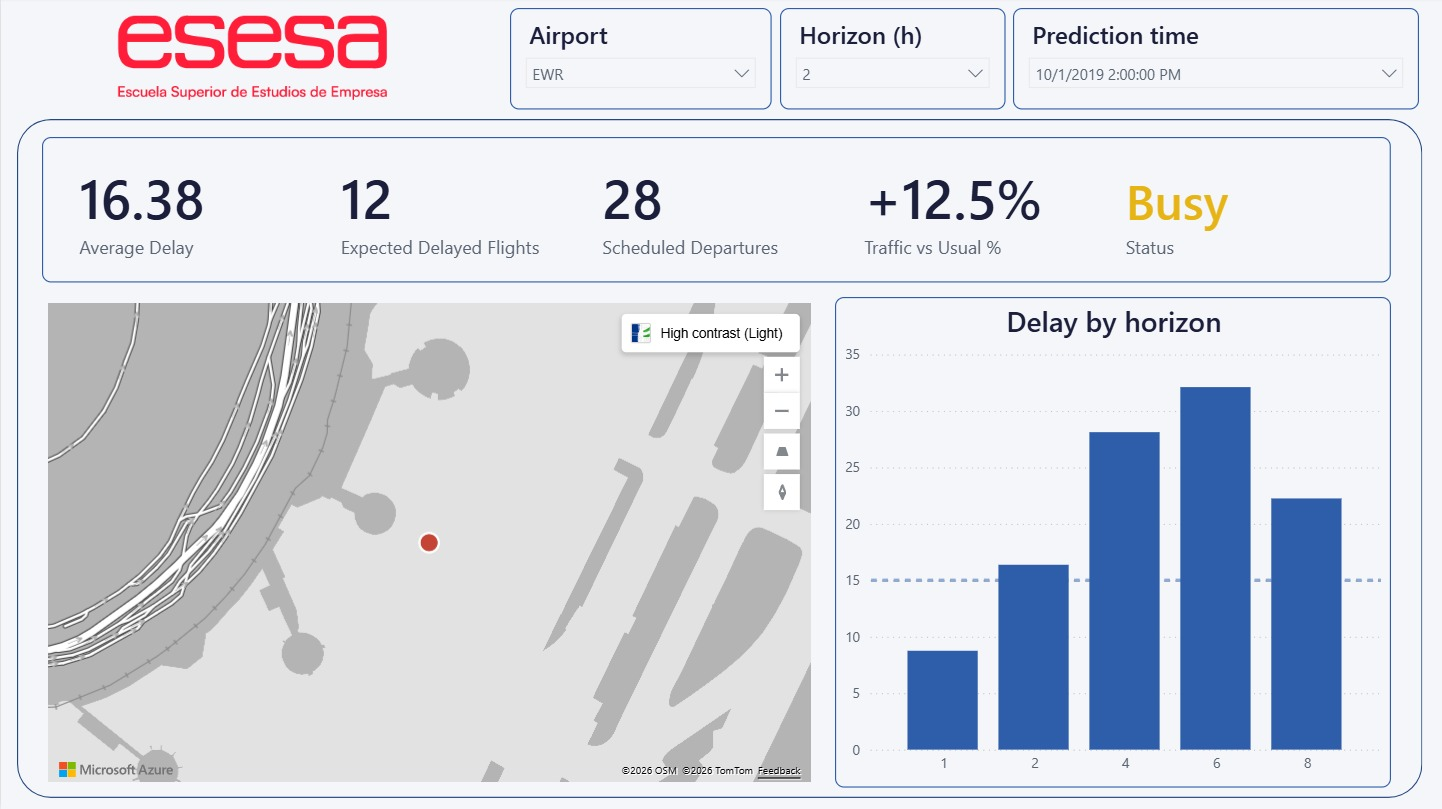
\includegraphics[width=\linewidth]{images/imgdashboard_aeropuerto_EWR.jpeg}
    \caption{Vista de aeropuerto individual: Newark Liberty International (EWR), horizonte de predicción de 2 horas, predicción generada a las 14:00 del 1 de octubre de 2019.}
    \label{fig:dashboard_ewr}
\end{figure}

\subsection{Vista de Aeropuerto Individual: Newark Liberty (EWR)}
\label{sub:vista_ewr}

La Figura~\ref{fig:dashboard_ewr} muestra el cuadro de mandos configurado para el aeropuerto de Newark Liberty International (código IATA: \textbf{EWR}), con un horizonte de predicción de \textbf{2 horas} y una marca temporal de predicción del 1 de octubre de 2019 a las 14:00. Esta vista es la más habitual en el uso operativo diario, ya que permite al gestor logístico centrar el análisis en el aeropuerto de origen o destino directamente relevante para su cadena de suministro.

\paragraph{KPIs de la cabecera.}
La banda superior de indicadores resume en una sola lectura el estado previsto del aeropuerto para el horizonte seleccionado:

\begin{itemize}
    \item \textbf{Average Delay: 16,38 min.} El retraso medio de llegada predicho por la Seq2SeqGNN para EWR en las próximas 2 horas supera el umbral operativo de referencia de 15 minutos (representado por la línea de puntos en el gráfico de barras), lo que activa automáticamente el estado de alerta en el sistema.
    \item \textbf{Expected Delayed Flights: 12.} La columna enriquecida \texttt{expected\_delayed\_flights}, calculada como el producto de la probabilidad de retraso predicha por la GNN ($\texttt{pct\_arr\_delayed\_15}$) y el volumen de llegadas programadas ($\texttt{sched\_arr\_count}$), estima que 12 de los 28 vuelos programados experimentarán un retraso superior a 15 minutos. Este indicador traduce la predicción probabilística del modelo en una magnitud de negocio directamente comprensible y accionable.
    \item \textbf{Scheduled Departures: 28.} Número de salidas programadas en la franja horaria analizada, extraído de los datos de Clase A (\textit{schedule}) del pipeline de ingesta. Proporciona contexto de volumen para interpretar el riesgo absoluto.
    \item \textbf{Traffic vs. Usual: +12,5\%.} Variación porcentual del tráfico en el bloque horario respecto al promedio histórico del mismo aeropuerto, día de la semana y franja horaria. Un valor positivo indica congestión superior a la habitual y es un predictor temprano de degradación de la puntualidad.
    \item \textbf{Status: Busy.} Indicador categórico tipo semáforo derivado de la combinación del retraso predicho y la desviación de tráfico. En este caso el estado \textit{Busy} (ámbar) señala riesgo moderado-alto: el sistema operativo está bajo presión pero no ha alcanzado el umbral de congestión severa (\textit{Critical}).
\end{itemize}



\paragraph{Gráfico de evolución del retraso por horizonte.}
El panel derecho presenta un gráfico de barras verticales con el retraso medio predicho ($\widehat{d}_h$) en el eje de ordenadas (minutos) para cada uno de los cinco horizontes de predicción $h \in \{1, 2, 4, 6, 8\}$ horas. La línea de puntos horizontal a 15 minutos actúa como umbral de referencia operativa estándar de la FAA (\textit{Federal Aviation Administration}).

El perfil temporal observado en EWR revela un patrón de congestión creciente: el retraso predicho asciende desde aproximadamente 9 minutos a 1 hora vista hasta un máximo de 32 minutos a 6 horas, para posteriormente descender a 23 minutos en el horizonte de 8 horas. Este patrón es típico de un evento de congestión en desarrollo, probablemente asociado a la acumulación de demora de aeronaves durante las horas punta del mediodía, con una recuperación parcial prevista hacia el final del día operativo.

% ----------------------------------------------------------
%  FIGURA 2 — Vista global (All airports, All horizons)
% ----------------------------------------------------------
\begin{figure}[H]
    \centering
    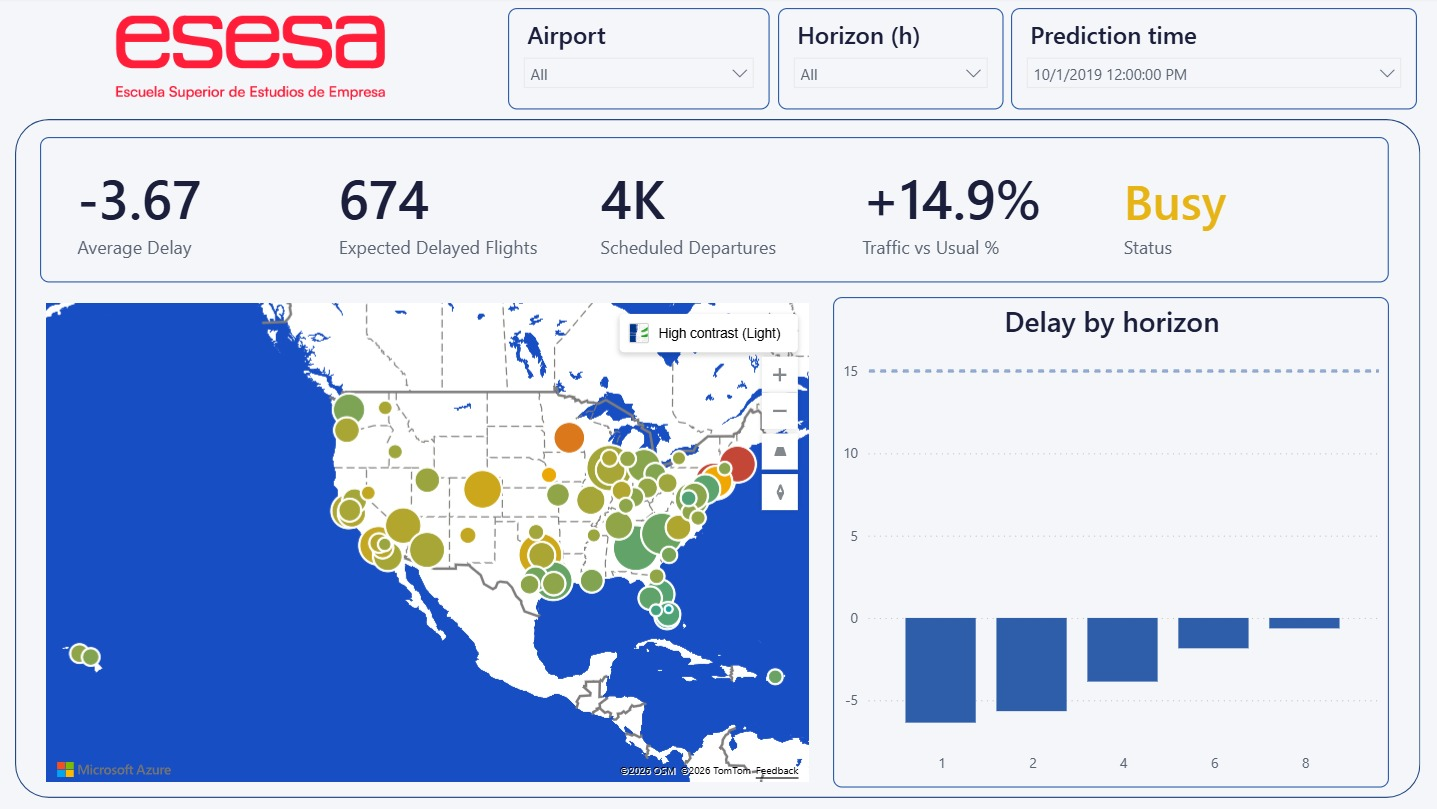
\includegraphics[width=\linewidth]{images/imgdashboard_global.jpeg}
    \caption{Vista global del sistema: todos los aeropuertos y horizontes, predicción generada a las 12:00 del 1 de octubre de 2019. El mapa de burbujas muestra la distribución geográfica de la congestión predicha con codificación de color y tamaño.}
    \label{fig:dashboard_global}
\end{figure}

\subsection{Vista Global del Sistema: Todos los Aeropuertos}
\label{sub:vista_global}

La Figura~\ref{fig:dashboard_global} presenta el cuadro de mandos en su modo de visión estratégica, con los filtros de aeropuerto y horizonte configurados a \textit{All} y la marca temporal establecida a las 12:00 del 1 de octubre de 2019. Esta vista está orientada al gestor de operaciones que necesita una fotografía instantánea del estado de toda la red aérea nacional antes de iniciar la jornada operativa.

\paragraph{KPIs agregados de la red nacional.}
La lectura agregada de los indicadores revela una situación aparentemente contradictoria que ilustra un matiz importante del modelo:

\begin{itemize}
    \item \textbf{Average Delay: $-$3,67 min.} El retraso medio ponderado sobre todos los aeropuertos y horizontes es negativo. Este valor no indica un error del sistema, sino que refleja el comportamiento real del tráfico aéreo a las 12:00: muchos vuelos del mediodía cierran puertas ligeramente antes de su hora programada (adelantos de 1 a 5 minutos son habituales cuando la carga de pasajeros permite un boarding rápido). El hecho de que el modelo capture este fenómeno de anticipación demuestra que la Seq2SeqGNN ha aprendido los patrones de distribución temporal real de los datos y no simplemente a predecir retrasos positivos.
    \item \textbf{Expected Delayed Flights: 674.} A pesar del retraso medio negativo, el número absoluto de vuelos con probabilidad de retraso $\geq 15$ minutos es de 674, lo que subraya que la métrica \texttt{expected\_delayed\_flights} es el indicador operativo más robusto: captura la cola derecha de la distribución de retrasos (los eventos severos) incluso cuando la media global es favorable.
    \item \textbf{Scheduled Departures: 4K.} El volumen total de salidas programadas en la franja horaria analizada alcanza los 4.000 vuelos, cifra coherente con la actividad del mediodía en el espacio aéreo estadounidense durante un día laborable de otoño.
    \item \textbf{Traffic vs. Usual: +14,9\%.} El incremento de tráfico respecto a la media histórica es superior al observado en la vista de EWR (+12,5\%), lo que sugiere que la presión de demanda es generalizada en toda la red y no un fenómeno local del área de Nueva York.
    \item \textbf{Status: Busy.} El estado de la red permanece en nivel de alerta ámbar (\textit{Busy}), coherente con la combinación de tráfico elevado y un número significativo de vuelos con riesgo de retraso severo, pese al retraso medio global negativo.
\end{itemize}

\paragraph{Mapa de burbujas con codificación semántica doble.}
El elemento visual más destacado de la vista global es el mapa de burbujas superpuesto sobre la cartografía de los Estados Unidos. Cada burbuja representa un aeropuerto de la red y su representación codifica dos dimensiones simultáneamente:

\begin{itemize}
    \item \textbf{Tamaño de la burbuja:} Proporcional al volumen de vuelos programados (\texttt{sched\_dep\_count}), de modo que los grandes \textit{hubs} (aeropuertos de Atlanta, Chicago, Dallas o Los Ángeles) aparecen visualmente dominantes, reflejando su peso real en la red.
    \item \textbf{Color de la burbuja:} Escala continua de verde (retraso bajo o negativo) a rojo (congestión severa), derivada del valor de \texttt{predicted\_arr\_delay\_min} normalizado. Esta doble codificación permite identificar de un vistazo los aeropuertos que combinan alto volumen con alto retraso predicho, que son precisamente los nodos críticos de la red con mayor capacidad de propagación del efecto dominó.
\end{itemize}

El patrón geográfico observable en la Figura~\ref{fig:dashboard_global} es coherente con el conocimiento experto de la operación aérea estadounidense: los aeropuertos del noreste (eje Boston--Nueva York--Washington) y del corredor Chicago--Detroit presentan burbujas de mayor tamaño y tonalidades más cálidas (naranja-rojo), reflejando la mayor densidad de tráfico y la mayor susceptibilidad a la congestión de la costa este durante las horas punta del mediodía.

\paragraph{Gráfico de evolución del retraso por horizonte (vista global).}
A diferencia del perfil creciente observado en EWR, el gráfico de barras en la vista global muestra retrasos negativos en todos los horizontes, que se aproximan asintóticamente a cero conforme el horizonte aumenta. Este patrón es estadísticamente coherente: a las 12:00 del mediodía, la mayoría de los vuelos del día todavía están en tierra con sus planes de vuelo originales, y la tendencia del modelo a predecir ligeros adelantos en la franja del mediodía refleja el comportamiento histórico de recuperación de tiempo en los vuelos cortos de enlace.


% ==========================================================
%         CAPÍTULO 6: CONCLUSIONES Y TRABAJO FUTURO
% ==========================================================
\chapter{Conclusiones y Trabajo Futuro}
\label{cap:conclusiones}

\section{Síntesis de Resultados}
\label{sec:sintesis}

El presente trabajo ha demostrado la viabilidad técnica y operativa de una arquitectura integral de Big Data y analítica predictiva aplicada a la gestión de retrasos aeroportuarios. El modelo se entrenó sobre datos históricos de la BTS de 2018--2019 (partición temporal: entrenamiento anterior a julio de 2019, test a partir de octubre de 2019), mientras que el feed en tiempo real se simula remapeando el año 2022, tal como se describe en el Capítulo~\ref{cap:ingenieria}. Los principales logros del proyecto se pueden sintetizar en tres dimensiones:

Desde la perspectiva de la \textbf{ingeniería de datos}, se ha diseñado e implementado un pipeline de extremo a extremo completamente automatizado sobre Microsoft Fabric, que combina una Azure Function serverless como punto de ingesta horaria, un rolling buffer con poda automática de particiones para gestionar la ventana deslizante, y notebooks de PySpark orquestados por pipelines de Data Factory. La separación de datos en Clase A (schedule) y Clase B (actuals) garantiza la integridad del experimento predictivo, evitando el \textit{data leakage} que comprometería la validez del modelo.

Desde la perspectiva del \textbf{modelado predictivo}, la arquitectura Seq2SeqGNN ha demostrado ser capaz de capturar simultáneamente la dimensión espacial (propagación de retrasos entre aeropuertos conectados) y la dimensión temporal (evolución de la red a lo largo de una secuencia de snapshots horarios). La cabeza multi-tarea con salidas de regresión (retraso en minutos) y clasificación binaria (probabilidad de retraso $\geq 15$ min) proporciona al sistema operativo las dos métricas que los gestores logísticos necesitan para tomar decisiones: magnitud esperada del retraso y certidumbre del mismo.

La Tabla~\ref{tab:resultados_mae} resume el rendimiento del modelo campeón
(\texttt{seq2seq\_gnn\_large}) sobre el conjunto de test. El modelo alcanza un MAE global
de 10,05 minutos en la predicción del retraso de llegada, con una degradación gradual y
controlada a medida que aumenta el horizonte de predicción --- comportamiento esperable y
deseable frente a los modelos autorregresivos, que acumulan error en cada paso. Este nivel
de error sitúa al sistema en un rango plenamente operativo y comparable al de los enfoques
publicados en la literatura de predicción de retrasos aéreos.

{\setlength{\intextsep}{16pt}
 \setlength{\abovecaptionskip}{6pt}   % space above the caption (paragraph -> caption)
 \setlength{\belowcaptionskip}{10pt}  % space below the caption (caption -> table)  <-- the gap you want
\begin{table}[h!]
\centering
\caption{Rendimiento del modelo Seq2SeqGNN campeón en el conjunto de test, por horizonte
de predicción. MAE y RMSE expresados en minutos.}
\label{tab:resultados_mae}
% \vspace{\baselineskip}   % <-- alternative to \belowcaptionskip: a literal blank line here
\begin{tabular}{@{}lcc@{}}
\toprule
\textbf{Horizonte} & \textbf{MAE (min)} & \textbf{RMSE (min)} \\
\midrule
$T+1$           & 9{,}07           & 16{,}36 \\
$T+2$           & 9{,}35           & 16{,}51 \\
$T+4$           & 10{,}09          & 18{,}36 \\
$T+6$           & 10{,}67          & 19{,}34 \\
$T+8$           & 11{,}05          & 20{,}90 \\
\midrule
\textbf{Global} & \textbf{10{,}05} & ---     \\
\bottomrule
\end{tabular}
\end{table}
}

Desde la perspectiva de la \textbf{inteligencia de negocio}, la conexión Direct Lake entre Delta Lake y Power BI elimina la latencia introducida por los procesos tradicionales de importación de datos, garantizando que el dashboard refleje siempre las predicciones más recientes sin intervención manual. El enriquecimiento de predicciones con volúmenes programados transforma las salidas abstractas del modelo en indicadores accionables como el número esperado de vuelos retrasados por aeropuerto y horizonte.

\section{Trabajo Futuro}
\label{sec:trabajo_futuro}

Las siguientes líneas de investigación y desarrollo representan extensiones naturales del sistema presentado:

\begin{itemize}
    \item \textbf{Integración de datos meteorológicos en tiempo real:} El modelo actual rellena el bloque meteorológico con ceros durante la inferencia en producción. La integración con una API meteorológica (por ejemplo, NOAA Aviation Weather Center) permitiría activar este bloque y potencialmente mejorar la precisión, especialmente en horizontes cortos donde el clima es el principal driver de retraso.
    \item \textbf{Aprendizaje continuo y reentrenamiento automático:} La tabla del historial \texttt{predictions\_history} acumula tanto las predicciones como los timestamps de ejecución. Cruzando estos datos con los actuals de Clase B con el desfase temporal correspondiente, es posible calcular el error real del modelo en producción y desencadenar un reentrenamiento automático cuando el rendimiento caiga por debajo de un umbral configurado.
    \item \textbf{Extensión de la cobertura geográfica:} El modelo actual cubre 70 aeropuertos de los Estados Unidos. La arquitectura es directamente escalable a redes de mayor tamaño (el espacio aéreo europeo, por ejemplo) sin cambios conceptuales, únicamente ajustando el mapa de aeropuertos y reentrenando con los datos correspondientes.
    \item \textbf{Predicción a nivel de vuelo individual:} La granularidad actual es a nivel de aeropuerto. Una extensión a nivel de vuelo individual requeriría modelar los nodos como vuelos (en lugar de aeropuertos) y las aristas como dependencias de aeronave, lo que aumentaría dramáticamente el tamaño del grafo pero proporcionaría predicciones directamente accionables a nivel operacional.
    \item \textbf{Integración con sistemas ERP/TMS:} La exportación de alertas desde Power BI hacia sistemas de planificación de recursos empresariales (ERP) o de gestión de transporte (TMS) cerraría el ciclo de valor del proyecto, permitiendo que las predicciones de retraso desencadenen automáticamente acciones correctivas en la cadena de suministro (por ejemplo, activar stock de seguridad o reasignar transportes terrestres).
\end{itemize}

\end{document}
